\documentclass{article}
%\usepackage[french]{babel}
\usepackage[utf8]{inputenc}
\usepackage{graphicx}
\usepackage{amsmath}
\usepackage{algorithm}
\usepackage[noend]{algpseudocode}

\makeatletter
\def\BState{\State\hskip-\ALG@thistlm}
\makeatother

\begin{document}
  
  \title{Continuous optimisation: \\
    \large The basu's problem}
  \author{PALLAMIDESSI Joseph, ERSFELD Thomas}
  \maketitle
  
  \section{Introduction} % (fold)
  \label{sec:Intr}
    \paragraph{} % (fold)
    \label{par:}
    The goal of this project is to provide a set of the 22 constants to the
    function derived from article\cite{} to fit a gaussian function of $\mu=1.5$ and
    $\phi=0.2$.

    %Gaussian
    % paragraph  (end)
  % section Intr (end)

  \section{Implementation} % (fold)
  \label{sec:Implementation}
    \subsubsection{Genome definition} % (fold)
    \label{ssub:Genome definition}
      
      \paragraph{} % (fold)
      \label{par:}
        The genome is defined as an array of 22 doubles, so each value is mapped to a
        specific product value as explained by the following table:
      % paragraph  (end)
      \\
      \\
      \scalebox{0.7}{ 
        \begin{tabular}{ |c |c |c |c |c |c |c |c |c |c |c |c}
          \hline                       
          1 & 2 & 3 & 4 & 5 & 6 & 7 & 8 & 9 & 10 & 11 \\ \hline                       
          kTR1 & KA1 &nA1&dmRNA1&kTL1&dLaclI&KTL1'&dCI&kTR2 & KR2 &nR2    \\
          \hline  
        \end{tabular}
      }
      \\
      \\
      \scalebox{0.7}{ 
        \begin{tabular}{ |c |c |c |c |c |c |c |c |c |c |c |c}
          \hline                       
          12 & 13 & 14 & 15 & 16 & 17 & 18 & 19 & 20 & 21 & 22  \\ \hline                       
          dmRNA2 & kTL2 & dLacl & kTR3 & KR3 & nR3 & KR3' & nR3' & dmRNA3 & kTL3 & dGFP  \\
          \hline  
        \end{tabular}
      }

      % The table 
      
      \paragraph{} % (fold)
      \label{par:}
        For the result of this report we will refer to each cell of the array
        (ie. parameter that we tried to optimize) as genes.
      % paragraph  (end)
    
    % subsubsection Genome definition (end)
    \subsubsection{Initialization} % (fold)
    \label{ssub:initialization}
      
      \paragraph{} % (fold)
      \label{par:}
        For each gene, we defined its bounds as given by this project subject.
        Here is a quick reminder:
      % paragraph  (end)
      
      \begin{figure}
      \begin{small} 
        \begin{tabular}{ | c |c | c |}
          \hline                       
            Parameter & min & max \\ \hline                       
            kTR1 &            0,001           &    1000000   \\ \hline    
            KA1 &             0,0001          &    1000 \\ \hline  
            nA1 &             1               &    4 \\ \hline
            dmRNA1 &          0,001           &    0,1 \\ \hline
            kTL1 &            0,0000001       &    0,00001 \\ \hline
            dLaclI &          0,0001          &    0,01 \\ \hline
            KTL1' &           0,0000001       &    0,00001 \\ \hline
            dCI &             0,0001          &    0,01 \\ \hline
            kTR2 &            0,001           &    1000000 \\ \hline
            KR2 &             0,0001          &    1000 \\ \hline
            nR2 &             1               &    4 \\ \hline
            dmRNA2 &          0,001           &    0,1 \\ \hline
            kTL2 &            0,0000001       &    0,00001 \\ \hline
            dLacl &           0,0001          &    0,01 \\ \hline
            kTR3 &            0,001           &    1000000 \\ \hline
            KR3 &             0,0001          &    1000 \\ \hline
            nR3 &             1               &    4 \\ \hline
            KR3' &            0,0001          &    1000 \\ \hline
            nR3' &            1               &    4 \\ \hline
            dmRNA3 &          0,001           &    0,1 \\ \hline
            kTL3 &            0,0000001       &    0,00001 \\ \hline
            dGFP &            0,0001          &    0,01i   \\ 
            \hline  
        \end{tabular}
      \end{small}
      \end{figure}
      % table of bounds

    % subsubsection initialization (end)

    \subsubsection{Evaluation} % (fold)
    \label{ssub:Evaluation}
      
      \paragraph{} % (fold)
      \label{par:}
        We decided to use a sample of the target function and the function to optimize
        with a sampling rate of 100, in the hope of having a very close approximation. 
        The fitness function used is a Root-mean-square deviation of the two vectors
        resulting from the sampling.
        \\
        \\
        RMSD = $\sqrt{\frac{\sum_{t=1}^n (x_{1,t} - x_{2,t})^2}{n}}$
      % paragraph  (end)

    % subsubsection Evaluation (end)
    
    \subsubsection{Crossover} % (fold)
    \label{ssub:Crossover}
      
      \paragraph{} % (fold)
      \label{par:}
      
        Since we are dealing with real value parameters, the crossover function
        is a simple barycentric one, which is commonly found in a lot of continous
        optimization genetic algorithms.
      % paragraph  (end)
      
      \begin{algorithm}
      \caption{Barycentric crossover}\label{pseudo1}
      \begin{algorithmic}[1]
      \Procedure{Crossover}{}
      \ForAll{gene in Genome}
        \State $alpha\gets random(0.,1.)$ 
        \State $Child.gene\gets alpha * Parent1.gene + (1. - alpha) * Parent2.gene$
      \EndFor
      \EndProcedure
      \end{algorithmic}
      \end{algorithm}

    
    % subsubsection Crossover (end)
    
    \subsubsection{Mutator} % (fold)
    \label{ssub:Mutator}
    
      \paragraph{} % (fold)
      \label{par:}
        Once again a simple technique was used. Given a constant mutation parameter,
        for each gene of the genome a chance is given to add or substract a random value
        within this mutation limit. We then avoid genes values going outside of their
        bounds by capping the values by the genes value bounds.
      % paragraph  (end)

      \begin{algorithm}
      \caption{Mutator operator}\label{pseudo2}
      \begin{algorithmic}[2]
      \Procedure{Mutator}{}
      \ForAll{gene in Genome}
        \If {$tossCoin(mutation_per_gene)$} 
          \State $alpha\gets random(-0.5, 0.5)$ 
          \State $Individual.gene\gets Individual.gene + alpha * Individual.gene$
          \State $Individual.gene\gets MAX(Individual.gene, gene.min)$
          \State $Individual.gene\gets MIN(Individual.gene, gene.max)$
        \EndIf
      \EndFor
      \EndProcedure
      \end{algorithmic}
      \end{algorithm}

    % subsubsection Mutator (end)
  % section Implementation (end)

  \section{Preliminary results} % (fold)
  \label{sec:Preliminaty Result}
    
    \paragraph{} % (fold)
    \label{par:}
      To much of our surprise, when we ran the optimization with an ahl concentration
      from 0.0001 to 10, the resulting function was quite bad. So bad, in fact, that
      we quickly realized that the optimized function was constant to the average of
      the gaussian values.
    % paragraph  (end)
    
    \paragraph{} % (fold)
    \label{par:}
      By empirecally modifying the range of ahl, we discover that given the basu's
      function definition, there was no way that with only one set of parameters we would
      obtain a good approximation on the whole definition range specified in the
      subject (i.e [0.0001,10]). 
    % paragraph  (end)

    \paragraph{} % (fold)
    \label{par:}
      However we did have some pretty good results on smaller definition range,
      fortunately, for the most interesting range of [1,1.8] as demonstrated by the
      following figure.
    % paragraph  (end)

    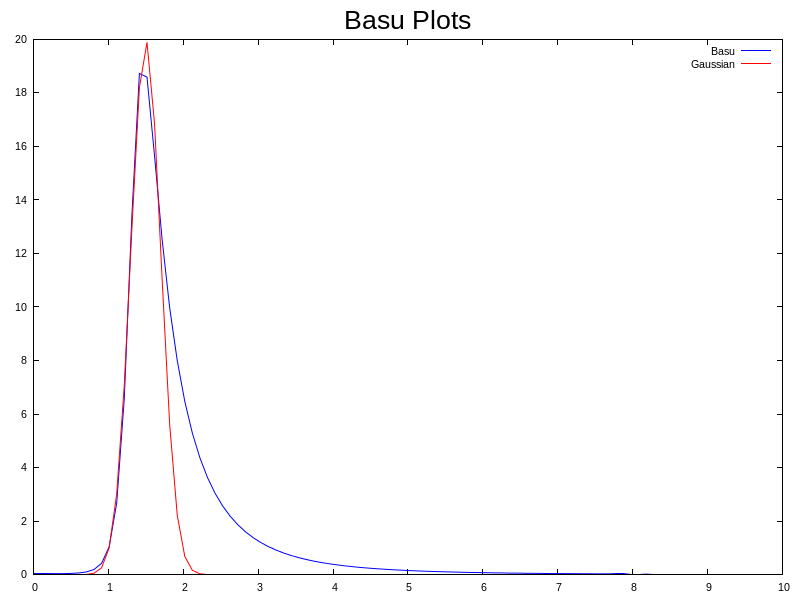
\includegraphics[scale=0.3]{basu_best}
    
  % section Result (end)
   
   \section{Results} % (fold)
   \label{sec:Result}
   \paragraph{} % (fold)
   
     \label{par:}
       Here are the observed results, averaged on 30 runs:
     % paragraph  (end)
    
    \begin{figure}
    \begin{small} 
    \begin{tabular}{lrrr}
      Parameter &  \\
      \hline
      Nb of generations & 2000 \\
      Population size & 2048  \\
      Crossover probability & 1 \\
      Mutation probability & 0.02\\
      Surviving parents & 100\%  \\
      Surviving offspring & 100\% \\
      Elitism & Strong \\
      Elite & 1 \\ \hline
      \emph{Result} & 1.17e+00 \\
      \hline 
      \end{tabular}
      \caption{Parameters for basu optimisation}
    \end{small}
    \end{figure}
   % section Result (end)

   \section{Further analysis and development} % (fold)
   \label{sec:section name}
   \paragraph{} % (fold)
   \label{par:}
   
   % paragraph  (end)
     In the end, we felt that multiple sets of parameters, by breaking the problem
     definition range into several continuous ones, must be used in order to have
     a good approximation of the target function.

   % section section name (end)
  

\end{document}
